%==================================================================%
% Author : Pando Muñoz, Manuel                                     %
% Sánchez Barreiro, Pablo                                          %
% Version: 1.0, 02/03/2011                                         %
%                                                                  %
% Memoria del Proyecto Fin de Carrera                              %
% Archivo raíz para el capítulo de iteración2                      %
%==================================================================%

\chapterheader{Segunda iteración}{Descripción de la segunda iteración}
\label{chap:iteracion2}


En el siguiente capítulo se describe lo realizado en la segunda iteración de construcción.
Se parte de lo obtenido en las iteraciones previas, que esta expuesto a lo largo de los capítulos precedentes.
\newline

En cuanto al estado de la aplicación, en la primera iteración de construcción, descrita en el capítulo \ref{chap:iteracion1}, se ha desarrollado un sistema distribuido, en el que el alumno puede conectarse con la aplicación del profesor y recibir ficheros enviados desde ella.
\newline

El objetivo de esta iteración es que el profesor pueda establecer el inicio y de la prueba, poder prefijar una hora de finalización de la misma y que la aplicación del alumno sea capaz de denegar el acceso a la red mientras dure la prueba.
\newline

En la tabla \ref{tabla:objetivosIteracion} se pueden ver los requisitos de alto nivel a implementar durante esta iteración, en la \ref{tabla:objetivosRefinadosIteracion} ya refinados y en la \ref{tabla:baseIteracion} la base, o lo que es lo mismo, lo implementado en la iteración anterior. La lista global de requisitos se encuentra en la tabla \ref{tabla:requisitos}.
\newline

\chaptertoc


\begin{table}
    \begin{tabular}{|c|p{10cm}|}
    \hline
    \textbf{Identificador} & \textbf{Descripción}
    \\ \hline

    R03 & El profesor debe ser capaz desde el \emph{Watchman} de indicar el inicio de la prueba.
    \\ \hline

    R05 & El profesor ha de ser capaz desde el \emph{Watchman} de establecer una hora límite para la duración de la prueba.
    \\ \hline

    R10 & El alumno desde su computador debe tener la posibilidad de ver el tiempo restante el pruebas de duración prefijada.
    \\ \hline

    R11 & La aplicación del alumno ha de ser capaz de denegar el acceso a la red al empezar la prueba.
    \\ \hline

    \end{tabular}
    \caption{Objetivos de la iteración}
    \label{tabla:objetivosIteracion}
\end{table}

\begin{table}
    \begin{tabular}{|c|p{10cm}|}
    \hline
    \textbf{Identificador} & \textbf{Descripción}
    \\ \hline

    R01 & Un computador de la red debe poder ser designado como \emph{Watchman}.
    \\ \hline

    R02 & Todos los computadores que no sean \emph{Watchman} serán computadores
    normales, y podrán ser utilizados para la realización de las pruebas evaluables.
    \\ \hline

    R06 & El profesor debe ser capaz desde el \emph{Watchman} de enviar el fichero de enunciado al resto de computadores.
    \\ \hline

    R07 & El alumno desde su computador debe ser capaz de conectarse al \emph{Watchman}.
    \\ \hline

    R13 & La aplicación ha de ser capaz de comprobar que los archivos se han enviado correctamente.
    \\ \hline

    \end{tabular}
    \caption{Requisitos ya implementados del sistema}
    \label{tabla:baseIteracion}
\end{table}



\begin{table}
    \begin{tabular}{|c|p{10cm}|}
    \hline
    \textbf{Identificador} & \textbf{Descripción}
    \\ \hline

    R03 & El profesor debe ser capaz desde el \emph{Watchman} de indicar el inicio de la prueba.
    \\ \hline

    R03.1 & Para que comience la prueba es necesario el nombre de la asignatura, el directorio dónde recibir resultados y una hora de finalización.
    \\ \hline

    R03.1.1 & Se han de tener privilegios de escritura en el directorio seleccionado.
    \\ \hline

    R03.2 & Se ha de pedir confirmación antes de comenzar realmente.
    \\ \hline

    R05 & El profesor ha de ser capaz desde el \emph{Watchman} de establecer una hora límite para la duración de la prueba.
    \\ \hline

    R05.1 & Si la hora de finalización es inferior a la del momento en que comienza la prueba, no se tendrá en cuenta.
    \\ \hline

    R10 & El alumno desde su computador debe tener la posibilidad de ver el tiempo restante el pruebas de duración prefijada.
    \\ \hline

    R10.1 & Se implementará con un hilo propio para no bloquear la interfaz.
    \\ \hline

    R11 & La aplicación del alumno ha de ser capaz de denegar el acceso a la red al empezar la prueba.
    \\ \hline

    R11.1 & Se utilizará iptables como medio para impedir el acceso a la red.
    \\ \hline

    R11.2 & Se utilizará un demonio para la interacción privilegiada con iptables.
    \\ \hline

    \end{tabular}
    \caption{Objetivos refinados de la iteración}
    \label{tabla:objetivosRefinadosIteracion}
\end{table}


\section{Incrementos realizados}

En las siguientes secciones se describen los incrementos realizados dentro de esta iteración, generalmente coincide el número de incrementos en cada iteración con el número de requisitos a implementar.

\subsection{Inicio de la prueba}
\label{sec:iteracion2:iniPrueba}

En esta sección se comenta cómo se consigue que el profesor pueda notificar a los alumnos el inicio de la prueba.
Como ya hemos comentado, partimos de la iteración anterior en la cual los alumnos eran capaces de conectar a la aplicación del profesor. En la aplicación del alumno, cuando se crea una conexión, se inicia a su vez un hilo de ejecución que se mantiene a la espera de recibir distintas órdenes provenientes del computador del profesor. De este modo se hace muy simple mantener desde la aplicación del profesor una lista de las conexiones abiertas con cada alumno y, al presionar el botón de iniciar la prueba, recorrer esa lista enviando la orden por cada conexión, de modo similar a como se transfiere un fichero, sección \ref{sec:iteracion1:envio}. Cuando cada una de las aplicaciones del alumno recibe esa orden, actúa en consecuencia.

\subsection{Examen temporizado}
\label{sec:iteracion2:examenTemporizado}

El profesor puede establecer una hora límite, llegada la cual, la prueba terminará automáticamente. Cuando el profesor define este límite en su aplicación y decide comenzar la prueba, se envía también si hay una hora de fin y, en caso afirmativo, cual es junto con la orden de comenzar la prueba. De este modo la aplicación del alumno puede mostrar una cuenta atrás con los minutos restantes para la finalización, para facilitar la referencia temporal tal como se muestra en la imagen \ref{fig:iteracion2:tiempoRestante}.

\begin{figure}
    \centering
    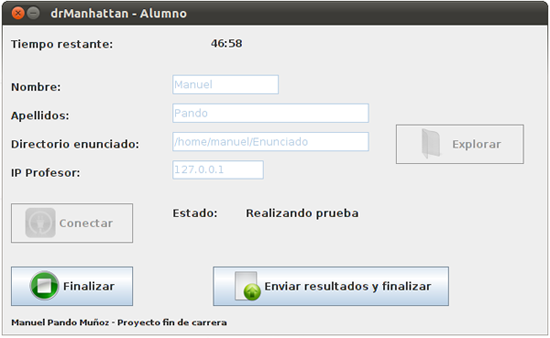
\includegraphics[width=.90\linewidth]{iteracion2/tiempoRestante}
    \caption{Aspecto de la GUI del alumno con una prueba temporizada.}
    \label{fig:iteracion2:tiempoRestante}
\end{figure}


\subsection{Denegar acceso a red}
\label{sec:iteracion2:denegarRed}

Cómo ya hemos visto en las secciones anteriores, una vez que la aplicación del alumno recibe la orden de comenzar la prueba, se ha de denegar el acceso a la red. Para ello se utiliza iptables, por medio de un demonio.
\newline

El demonio creado es muy simple, se ejecuta en segundo plano esperando a que la aplicación del alumno conecte, y en función de lo requerido en ese momento, permitir o no el acceso a la red interactuando con iptables. Este demonio se inicia en tiempo de arranque y con los permisos necesarios para poder usar el cortafuegos.
\newline

Las órdenes concretas que ejecuta el demonio son, cuándo se desea denegar la red:

\begin{center}

    iptables -P OUTPUT DROP

    iptables -A OUTPUT -s 127.0.0.1 -j ACCEPT

\end{center}

Con la primera de ellas se cambia la política del tratamiento a los paquetes salientes del equipo, de modo que los deseche, dicho de otro modo, no se permiten las comunicaciones salientes con otros computadores, de esta forma se evita que se hagan peticiones, por ejemplo, a un servidor web\cite{WEB:1996}.
\newline

La segunda es para permitir los paquetes salientes dirigidos al propio equipo local. Esto es necesario para la comunicación entre la aplicación del alumno y el demonio, que como se ha visto en la sección \ref{sec:arquitectura:arqLogica} se ejecutan en el mismo computador.
\newline

Puede parecer que el equipo queda totalmente aislado, incluso del computador del profesor, pero esto no es así, puesto que ya hay una conexión establecida y dado que la aplicación del alumno espera órdenes de la aplicación del profesor, puede seguir funcionando perfectamente, puesto que los paquetes de entrada sí que están permitidos, lo que estas instrucciones imposibilitan es la creación de nuevas conexiones y el envío de mensajes a cualquier computador que no sea el propio.


\section{Pruebas}
\label{sec:iteracion2:pruebas}


En esta sección se describen las pruebas realizadas en la iteración con el objetivo de determinar si el funcionamiento de lo construido es correcto.
\newline

\begin{itemize}

    \item {\bfseries R03} - El profesor debe ser capaz desde el \emph{Watchman} de indicar el inicio de la prueba.

    \begin{itemize}

        \item Prueba: Pulsar el botón para iniciar la prueba con alumnos conectados.
        \item Objetivo: A los alumnos conectados les llega la señal, no admite nuevas conexiones.

        \item Prueba: Pulsar el botón para iniciar la prueba sin alumnos conectados.
        \item Objetivo: Se inicia la prueba, no admite nuevas conexiones.

    \end{itemize}

    \item {\bfseries R05} - El profesor ha de ser capaz desde el \emph{Watchman} de establecer una hora límite para la duración de la prueba.

    \item {\bfseries R10} - El alumno desde su computador debe tener la posibilidad de ver el tiempo restante el pruebas de duración prefijada.

    \begin{itemize}
        \item Prueba: Establecer como límite temporal horas futuras y comenzar la prueba.
        \item Objetivo: La aplicación del alumno muestra el tiempo restante correcto. No se admiten nuevas conexiones.

        \item Prueba Establecer como límite temporal horas pasadas.
        \item Objetivo: Se inicia la prueba, la aplicación del alumno no muestra límite temporal. No se admiten nuevas conexiones.

        \item Prueba: Establecer como límite temporal horas incorrectas y comenzar la prueba.
        \item Objetivo: La aplicación del alumno detecta las horas erróneas y no comienza la prueba.
    \end{itemize}


    \item {\bfseries R11} - La aplicación del alumno ha de ser capaz de denegar el acceso a la red al empezar la prueba.

    \begin{itemize}

        \item Prueba: Después de que de inicio una prueba, en el computador del alumno, intentar abrir páginas web en el navegador, pings a equipos.
        \item Objetivo: La aplicación del alumno desactiva el acceso a la red.
    \end{itemize}

\end{itemize}

Como se puede comprobar tras la lectura de los dos capítulos dedicados a describir una iteración, la construcción en esta metodología es un proceso repetitivo y todas las iteraciones son muy similares. 


\section{Sumario}

En este capítulo, como en el anterior, se muestra el proceso a seguir de acuerdo a la metodología escogida, demostrando que es un proceso repetitivo. En el siguiente capítulo se describirán las acciones de despliegue y aceptación realizadas. 